\documentclass[10pt]{article}

\usepackage[utf8]{inputenc}
\usepackage[margin=0.75in]{geometry}
\usepackage{graphicx}
\usepackage{booktabs}
\usepackage{amsmath}
\usepackage{amssymb}
\usepackage{xcolor}
\usepackage{array}
\usepackage{caption}

% Enhanced (v2) supplement. Generated figures live in supplementary_assets_v2/;
% the original review figures remain in supplementary_assets/. Both are on the path.
\graphicspath{{supplementary_assets_v2/}{supplementary_assets/}}
\captionsetup{font=small,labelfont=bf}

\newcommand{\pp}{percentage points}

\begin{document}

\begin{center}
{\Large \textbf{Supplementary Material}}\\[0.4em]
{\large \textbf{MAML-Select: An Online Adaptive Client Selection Method for Federated Learning via Meta-Learning}}\\[0.3em]
{\normalsize \textit{Enhanced revision supplement (v2)}}
\end{center}

\section*{S1. Scope of the Supplement}

This supplement reports the additional evidence assembled during the revision. The main letter keeps the compact convergence and trade-off evidence, the $\lambda$-sensitivity plot, the feature-ablation plot, and the core tables. Here we expand on three fronts that strengthen reproducibility and reviewer confidence: (i) a complete experimental-setup and reproducibility section (S2); (ii) a full per-method benchmark reported with dispersion on \emph{every} metric (S3) together with paired effect sizes and confidence intervals (S4); and (iii) additional diagnostic visualizations---cumulative-resource and fairness trajectories (S5), accuracy--cost frontiers, and per-seed reproducibility plots (S6). Sensitivity, ablation, and overhead tables (S7) are retained, and we close with an explicit limitations statement (S8) and an interpretation of the revised claims (S9).

All results use the same non-IID setting as the main manuscript: $N=100$ clients, $K=10$ sampled per round, $E=5$ local epochs, batch size $32$, a Dirichlet label partition with $\alpha=0.5$, and seeds $42$, $123$, and $2026$ unless a table explicitly reports a smaller $n$. CIFAR-100 is analyzed at $150$ rounds so that CriticalFL is included without imputation. \textbf{No missing seeds or crashed runs are imputed}: where a method did not complete (e.g.\ CriticalFL on Fashion-MNIST and CIFAR-10), the corresponding cells are left blank. Energy and carbon are model-based estimates derived from the device-tier cost model and a declared grid intensity (S2), not hardware-meter readings.

\section*{S2. Experimental Setup and Reproducibility}

Table~\ref{tab:supp_config} lists the training and selector configuration, and Table~\ref{tab:supp_tiers} lists the device-heterogeneity model. The MAML-Select policy is the small $6$--$64$--$64$--$1$ multilayer perceptron ($4{,}673$ parameters) described in the main letter; its query loss is adapted with one inner gradient step of size $\beta$ and the outer policy is updated with Adam.

\begin{table}[!ht]
\centering
\caption{Training and MAML-Select selector configuration shared by all benchmark runs.}
\label{tab:supp_config}
\small
\begin{tabular}{@{}ll@{}}
\toprule
Component & Setting \\
\midrule
Clients $N$ / sampled per round $K$ & $100$ / $10$ \\
Communication rounds $T$ & $200$ (CIFAR-100 evaluated to $150$) \\
Local epochs $E$ / batch size & $5$ / $32$ \\
Client learning rate & $0.01$ with cosine annealing \\
Data partition & Dirichlet, $\alpha=0.5$ (non-IID) \\
Backbone models & LightCNN-9 (Fashion-MNIST); ResNet-18 (CIFAR-10/100) \\
\midrule
Selector policy & MLP $6$--$64$--$64$--$1$ ($4{,}673$ parameters) \\
Inner adaptation rate $\beta$ & $0.01$ (one look-ahead step) \\
Outer optimizer & Adam, $\eta=0.001$ \\
Latency--loss trade-off weight $\lambda$ & $0.5$ (selected operating point) \\
\midrule
Seeds & $42$, $123$, $2026$ \\
Declared grid intensity & $475$~g\,CO$_2$/kWh (India) \\
\bottomrule
\end{tabular}
\end{table}

\begin{table}[!ht]
\centering
\caption{Three-tier device-heterogeneity model. Compute speed is the relative local-processing rate (higher is faster); power and battery scale with capability. Tiers are assigned once per run by a seeded shuffle.}
\label{tab:supp_tiers}
\small
\begin{tabular}{@{}lrrrr@{}}
\toprule
Tier & Share of clients & Compute speed & Power (W) & Battery (Wh) \\
\midrule
Tier~1 (low-end)  & $20\%$ & $1.0\times$ & $4$  & $18$ \\
Tier~2 (mid-range) & $50\%$ & $2.0\times$ & $7$  & $30$ \\
Tier~3 (high-end) & $30\%$ & $4.0\times$ & $12$ & $48$ \\
\bottomrule
\end{tabular}
\end{table}

\paragraph{Resource model.} For each selected client $i$ the simulator models local wall-clock time as $t_i = E\,|\mathcal{D}_i|/v_i + \tau^{\text{comm}}_i$, where $v_i$ is the tier compute speed and $\tau^{\text{comm}}_i$ is the modeled communication time. Modeled energy is $e_i = (P_i/3600)\,t_i$~Wh with tier power $P_i$; per-round energy is $\sum_i e_i$ and per-round wall-clock is $\max_i t_i$ (straggler-bound). Carbon is $e\,(\text{Wh})/1000 \times 475$~g using the declared India grid intensity. Training compute (TFLOPs) accumulates model FLOPs over sampled clients, epochs, and samples. Because every selector samples exactly $K=10$ clients per round, per-round \emph{communication} is identical across selectors; resource savings therefore arise from \emph{which} clients are trained (compute, energy, carbon), not from bandwidth.

\section*{S3. Full Benchmark with Dispersion}

Table~\ref{tab:supp_full_benchmark} reports every method on every dataset with mean~$\pm$~s.d.\ across the available seeds, including the F1, communication, and coverage columns omitted from the compact main-letter table. CriticalFL completed only on CIFAR-100 (the longest-running setting); its Fashion-MNIST and CIFAR-10 cells are blank because those runs crashed and are not imputed. TiFL and FedCor contribute $n=1$ on CIFAR-100 and are shown without a dispersion term, as flagged by the $n$ column.

\begin{table}[!ht]
\centering
\caption{Full benchmark across datasets and methods (mean~$\pm$~s.d.; $n$ = completed seeds). Blank cells denote runs that did not complete and are \emph{not} imputed. Communication is byte-identical across selectors except for CriticalFL, whose sparsified uplink changes its payload.}
\label{tab:supp_full_benchmark}
\footnotesize
\resizebox{\textwidth}{!}{%
\begin{tabular}{@{}llrrrrrrrrr@{}}
\toprule
Dataset & Method & Acc. (\%) & F1 (\%) & TFLOPs & Energy (Wh) & Carbon (g) & Comm. (MB) & Jain & Coverage (\%) & $n$ \\
\midrule
Fashion-MNIST & FedAvg & 90.22$\pm$0.58 & 90.22$\pm$0.51 & 139.70$\pm$1.13 & 5752.10$\pm$72.27 & 2732.25$\pm$34.33 & 5631.99$\pm$0.00 & 0.95$\pm$0.00 & 100.00$\pm$0.00 & 3 \\
 & FedCS & 84.11$\pm$1.82 & 83.91$\pm$1.98 & 75.66$\pm$6.74 & 2771.73$\pm$210.62 & 1316.57$\pm$100.04 & 5631.99$\pm$0.00 & 0.10$\pm$0.00 & 10.00$\pm$0.00 & 3 \\
 & Oort & 86.70$\pm$0.19 & 86.42$\pm$0.26 & 148.83$\pm$8.10 & 5962.71$\pm$455.92 & 2832.29$\pm$216.56 & 5631.99$\pm$0.00 & 0.10$\pm$0.00 & 10.00$\pm$0.00 & 3 \\
 & TiFL & 86.73$\pm$0.34 & 86.51$\pm$0.34 & 146.86$\pm$6.41 & 6061.70$\pm$348.39 & 2879.31$\pm$165.48 & 5631.99$\pm$0.00 & 0.11$\pm$0.00 & 12.00$\pm$0.00 & 3 \\
 & FedCor & 89.35$\pm$0.50 & 89.22$\pm$0.57 & 120.53$\pm$4.92 & 4844.67$\pm$204.30 & 2301.22$\pm$97.04 & 5631.99$\pm$0.00 & 0.26$\pm$0.04 & 48.67$\pm$8.14 & 3 \\
 & CriticalFL & -- & -- & -- & -- & -- & -- & -- & -- & -- \\
 & FedGCS & 90.65$\pm$0.29 & 90.63$\pm$0.26 & 135.77$\pm$3.53 & 5595.01$\pm$112.93 & 2657.63$\pm$53.64 & 5631.99$\pm$0.00 & 0.95$\pm$0.02 & 100.00$\pm$0.00 & 3 \\
 & MAML-Select & 90.11$\pm$0.47 & 90.04$\pm$0.30 & 121.77$\pm$1.89 & 4808.53$\pm$78.68 & 2284.05$\pm$37.37 & 5631.99$\pm$0.00 & 0.77$\pm$0.06 & 100.00$\pm$0.00 & 3 \\
\midrule
CIFAR-10 & FedAvg & 79.43$\pm$1.84 & 79.36$\pm$1.78 & 8340.81$\pm$51.79 & 4797.50$\pm$24.10 & 2278.81$\pm$11.45 & 170354.64$\pm$0.00 & 0.95$\pm$0.00 & 100.00$\pm$0.00 & 3 \\
 & FedCS & 50.45$\pm$2.57 & 49.87$\pm$2.33 & 4080.75$\pm$600.04 & 2073.22$\pm$262.47 & 984.78$\pm$124.68 & 170354.64$\pm$0.00 & 0.10$\pm$0.00 & 10.00$\pm$0.00 & 3 \\
 & Oort & 60.19$\pm$5.18 & 59.69$\pm$4.61 & 8303.14$\pm$1923.10 & 4677.04$\pm$855.53 & 2221.59$\pm$406.38 & 170354.64$\pm$0.00 & 0.10$\pm$0.00 & 10.00$\pm$0.00 & 3 \\
 & TiFL & 61.93$\pm$5.04 & 61.36$\pm$4.60 & 8200.20$\pm$2143.28 & 4799.76$\pm$1203.46 & 2279.88$\pm$571.64 & 170354.64$\pm$0.00 & 0.11$\pm$0.00 & 12.00$\pm$0.00 & 3 \\
 & FedCor & 67.20$\pm$5.33 & 66.81$\pm$5.37 & 7748.45$\pm$695.13 & 4451.65$\pm$434.60 & 2114.54$\pm$206.44 & 170354.64$\pm$0.00 & 0.20$\pm$0.02 & 31.33$\pm$4.93 & 3 \\
 & CriticalFL & -- & -- & -- & -- & -- & -- & -- & -- & -- \\
 & FedGCS & 77.88$\pm$1.75 & 77.69$\pm$1.54 & 7655.60$\pm$277.86 & 4428.06$\pm$153.59 & 2103.33$\pm$72.96 & 170354.64$\pm$0.00 & 0.90$\pm$0.03 & 100.00$\pm$0.00 & 3 \\
 & MAML-Select & 75.63$\pm$1.43 & 75.25$\pm$1.34 & 6548.65$\pm$118.06 & 3610.06$\pm$60.14 & 1714.78$\pm$28.57 & 170354.64$\pm$0.00 & 0.61$\pm$0.01 & 100.00$\pm$0.00 & 3 \\
\midrule
CIFAR-100 & FedAvg & 59.66$\pm$0.29 & 59.13$\pm$0.40 & 6331.32$\pm$5.76 & 3626.16$\pm$18.10 & 1722.43$\pm$8.60 & 129260.25$\pm$0.00 & 0.94$\pm$0.00 & 100.00$\pm$0.00 & 3 \\
 & FedCS & 27.52$\pm$0.29 & 26.39$\pm$0.09 & 5334.17$\pm$23.23 & 2659.37$\pm$11.97 & 1263.20$\pm$5.68 & 129260.25$\pm$0.00 & 0.10$\pm$0.00 & 10.00$\pm$0.00 & 2 \\
 & Oort & 29.41$\pm$1.73 & 28.13$\pm$1.73 & 5955.29$\pm$188.55 & 3421.40$\pm$180.97 & 1625.16$\pm$85.96 & 129260.25$\pm$0.00 & 0.10$\pm$0.00 & 10.00$\pm$0.00 & 2 \\
 & TiFL & 32.12 & 31.02 & 5986.05 & 3499.35 & 1662.19 & 129260.25 & 0.11 & 12.00 & 1 \\
 & FedCor & 34.18 & 32.93 & 6427.86 & 3667.94 & 1742.27 & 129260.25 & 0.12 & 14.00 & 1 \\
 & CriticalFL & 48.84$\pm$1.58 & 48.07$\pm$2.32 & 9469.17$\pm$391.96 & 5438.48$\pm$213.92 & 2583.28$\pm$101.61 & 168380.73$\pm$6658.34 & 0.97$\pm$0.00 & 100.00$\pm$0.00 & 2 \\
 & FedGCS & 58.66$\pm$0.11 & 58.08$\pm$0.20 & 6140.38$\pm$24.35 & 3526.12$\pm$4.44 & 1674.91$\pm$2.11 & 129260.25$\pm$0.00 & 0.82$\pm$0.02 & 100.00$\pm$0.00 & 2 \\
 & MAML-Select & 58.15$\pm$0.51 & 57.66$\pm$0.33 & 6223.53$\pm$19.58 & 3456.51$\pm$6.06 & 1641.84$\pm$2.88 & 129260.25$\pm$0.00 & 0.78$\pm$0.03 & 100.00$\pm$0.00 & 3 \\
\bottomrule
\end{tabular}%
}
\end{table}

Three points stand out and are consistent with the cautious framing of the main letter. (i) MAML-Select is statistically close to the strongest accuracy baselines on Fashion-MNIST ($90.11$ vs.\ FedAvg $90.22$, FedGCS $90.65$) and CIFAR-100 ($58.15$ vs.\ FedAvg $59.66$, FedGCS $58.66$), while spending less modeled compute and energy. (ii) On CIFAR-10 it is deliberately \emph{below} FedAvg ($75.63$ vs.\ $79.43$, $-3.81$~\pp): this is the efficiency--accuracy trade-off the paper claims, not a win. (iii) CriticalFL, the only method that reaches competitive CIFAR-100 accuracy other than FedAvg/FedGCS, does so at the highest resource cost in the table ($9{,}469$~TFLOPs and $5{,}438$~Wh, versus $6{,}224$~TFLOPs and $3{,}457$~Wh for MAML-Select).

\section*{S4. Statistical Analysis: MAML-Select vs.\ FedAvg}

Table~\ref{tab:supp_maml_vs_fedavg} summarizes the paired resource reductions, and Table~\ref{tab:supp_stats} reports the full paired comparison---signed difference, $95\%$ confidence interval, the standardized paired effect size (Cohen's $d_z$), and the two-sided paired $p$-value---over the shared seeds. All differences are computed as MAML-Select minus FedAvg, so a negative value means MAML-Select is lower.

\begin{table}[!ht]
\centering
\caption{MAML-Select relative to FedAvg over shared seeds. Positive reductions indicate lower resource use for MAML-Select; $\Delta$Acc.\ is signed.}
\label{tab:supp_maml_vs_fedavg}
\small
\begin{tabular}{@{}lrrrrr@{}}
\toprule
Dataset & $\Delta$Acc. (pp) & TFLOPs $\downarrow$ (\%) & Energy $\downarrow$ (\%) & Carbon $\downarrow$ (\%) & $n$ \\
\midrule
Fashion-MNIST & -0.11 & 12.8 & 16.4 & 16.4 & 3 \\
CIFAR-10 & -3.81 & 21.5 & 24.7 & 24.7 & 3 \\
CIFAR-100 & -1.51 & 1.7 & 4.7 & 4.7 & 3 \\
\bottomrule
\end{tabular}
\end{table}

\begin{table}[!ht]
\centering
\caption{Paired comparison of MAML-Select against FedAvg over shared seeds ($n=3$). Differences are MAML-Select minus FedAvg (negative $=$ MAML-Select lower). $d_z$ is the standardized paired effect size; $p$ is a two-sided paired $t$-test. Communication is byte-identical ($\Delta=0$), so its interval and effect size are undefined.}
\label{tab:supp_stats}
\small
\begin{tabular}{@{}llrrrr@{}}
\toprule
Dataset & Metric & $\Delta$ (mean) & 95\% CI & Cohen's $d_z$ & $p$ \\
\midrule
Fashion-MNIST & $\Delta$Acc. (pp) & -0.11 & [-2.24, 2.02] & -0.13 & 0.840 \\
 & $\Delta$TFLOPs & -17.93 & [-25.44, -10.42] & -5.93 & 0.009 \\
 & $\Delta$Energy (Wh) & -943.58 & [-1291.09, -596.06] & -6.74 & 0.007 \\
 & $\Delta$Carbon (g) & -448.20 & [-613.27, -283.13] & -6.74 & 0.007 \\
 & $\Delta$Comm. (MB) & 0.00 & -- & -- & -- \\
 & $\Delta$Jain & -0.18 & [-0.32, -0.04] & -3.21 & 0.031 \\
\midrule
CIFAR-10 & $\Delta$Acc. (pp) & -3.81 & [-7.24, -0.37] & -2.75 & 0.041 \\
 & $\Delta$TFLOPs & -1792.16 & [-2143.33, -1440.99] & -12.68 & 0.002 \\
 & $\Delta$Energy (Wh) & -1187.44 & [-1350.37, -1024.52] & -18.11 & 0.001 \\
 & $\Delta$Carbon (g) & -564.04 & [-641.42, -486.65] & -18.11 & 0.001 \\
 & $\Delta$Comm. (MB) & 0.00 & -- & -- & -- \\
 & $\Delta$Jain & -0.35 & [-0.38, -0.32] & -28.54 & 0.000 \\
\midrule
CIFAR-100 & $\Delta$Acc. (pp) & -1.51 & [-2.84, -0.19] & -2.84 & 0.039 \\
 & $\Delta$TFLOPs & -107.80 & [-159.77, -55.82] & -5.15 & 0.012 \\
 & $\Delta$Energy (Wh) & -169.65 & [-208.36, -130.94] & -10.89 & 0.003 \\
 & $\Delta$Carbon (g) & -80.58 & [-98.97, -62.19] & -10.89 & 0.003 \\
 & $\Delta$Comm. (MB) & 0.00 & -- & -- & -- \\
 & $\Delta$Jain & -0.16 & [-0.23, -0.09] & -5.61 & 0.010 \\
\bottomrule
\end{tabular}
\end{table}

The resource reductions are both large and consistent: every compute, energy, and carbon difference is negative with a large standardized effect size ($|d_z| > 5$ in most cells) and $p < 0.05$. The accuracy picture is appropriately nuanced: on Fashion-MNIST the accuracy gap is negligible and \emph{not} significant ($-0.11$~\pp, $p=0.84$), whereas the CIFAR-10 and CIFAR-100 gaps are small but significant, confirming the trade-off rather than hiding it. The fairness rows are reported with the same transparency: MAML-Select's Jain index is significantly \emph{below} FedAvg on all three datasets, which is why the paper does not claim fairness superiority. With only three seeds the confidence intervals are necessarily wide; we report them precisely so that the strength of the resource effect---and the modesty of the accuracy effect---can be judged honestly.

\section*{S5. Convergence and Resource Trajectories}

Figure~\ref{fig:supp_convergence_all} shows all-dataset accuracy convergence. Figures~\ref{fig:supp_resource_traj} and~\ref{fig:supp_fairness_traj} are new round-resolved views: the first shows that MAML-Select's compute/energy/carbon advantage \emph{accumulates monotonically} over training rather than appearing only at the final round; the second shows the participation dynamics behind the fairness numbers. The expanded resource grid and accuracy--energy cross-checks (Figs.~\ref{fig:supp_resource_grid}--\ref{fig:supp_accuracy_energy}) are retained from the first revision.

\begin{figure}[!ht]
\centering
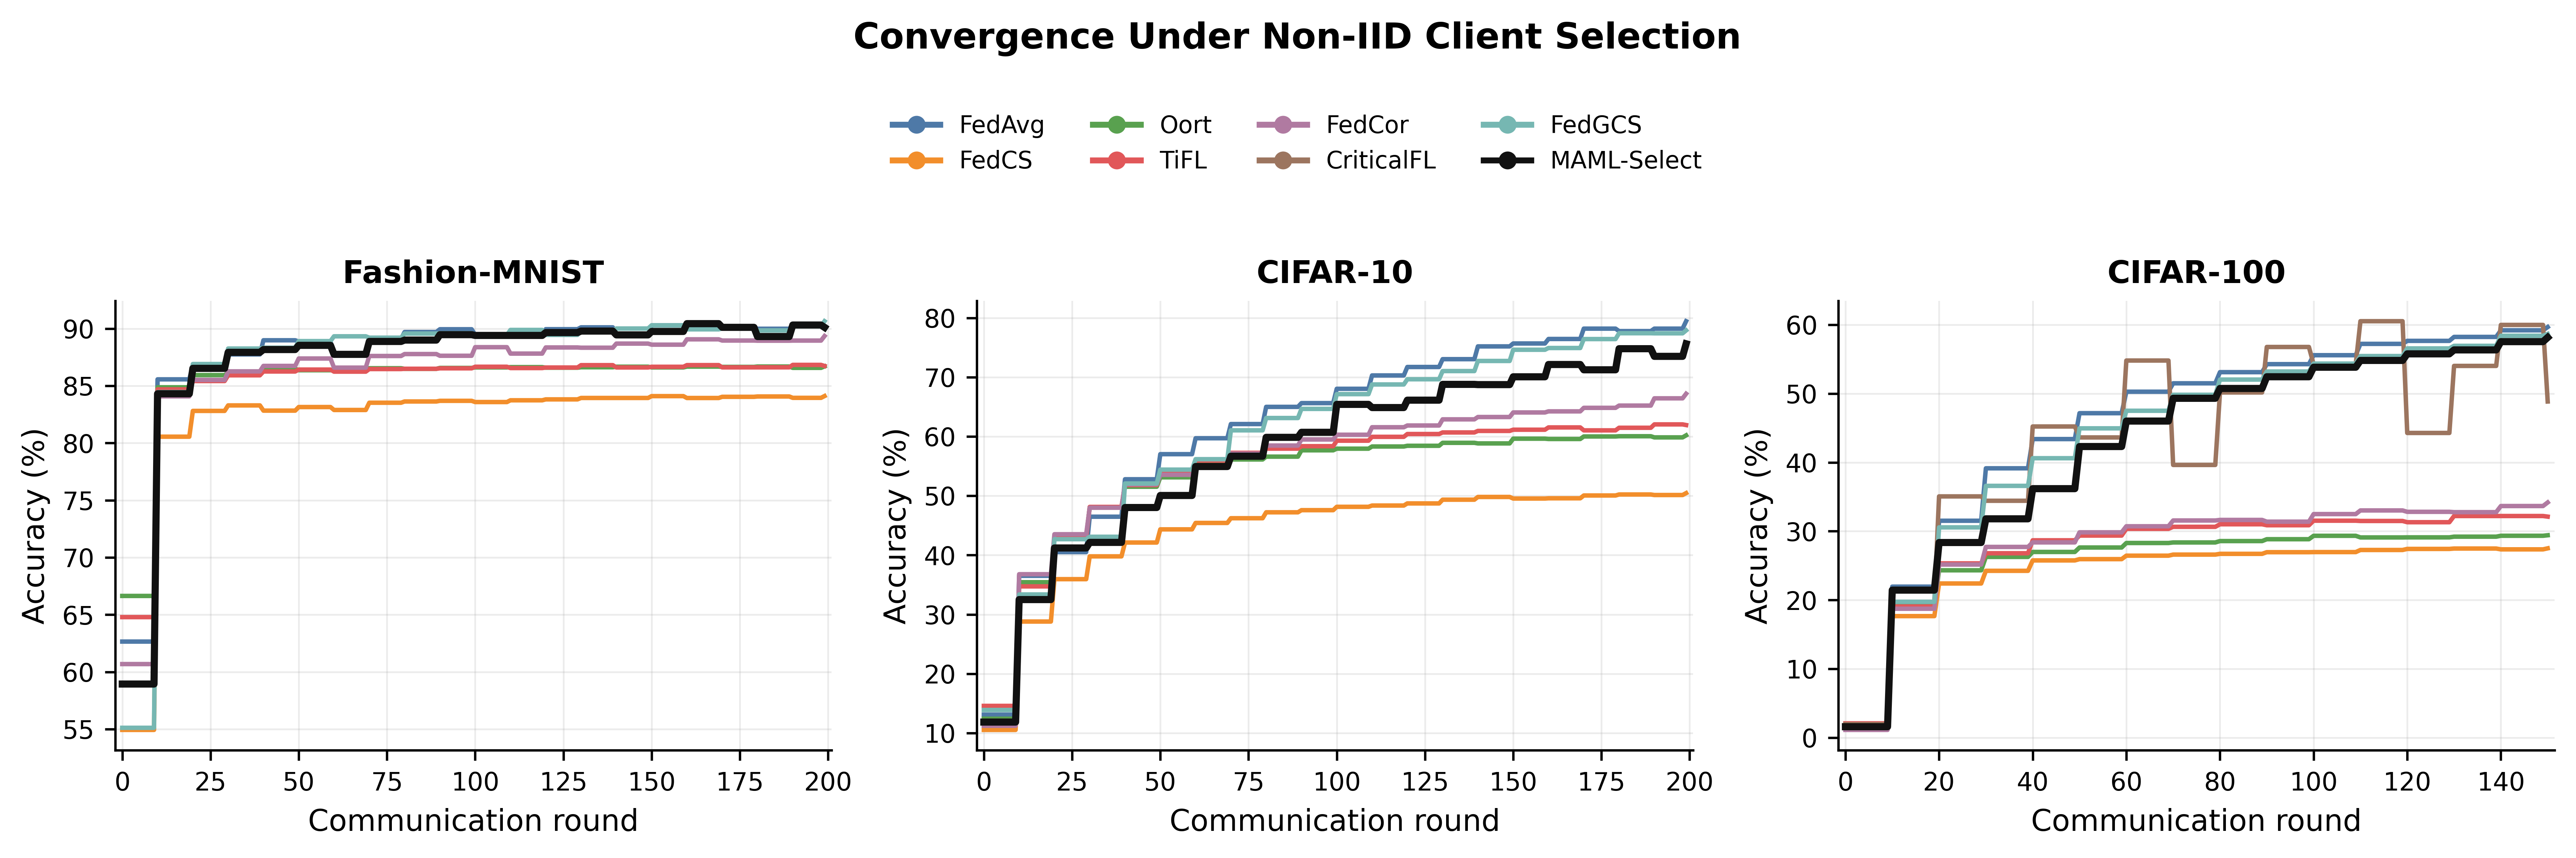
\includegraphics[width=0.94\textwidth]{review_fig_convergence_all_datasets.png}
\caption{All-dataset convergence summary used to check consistency before curating the main-letter figures. The main paper reports the final CIFAR-100 four-panel version because it is the hardest setting and includes CriticalFL.}
\label{fig:supp_convergence_all}
\end{figure}

\begin{figure}[!ht]
\centering

\includegraphics[width=0.98\textwidth]{supp_resource_trajectories.png}
\caption{Cumulative compute (TFLOPs), modeled energy (Wh), and modeled carbon (g) versus communication round, averaged over seeds; the shaded band is $\pm1$~s.d.\ for MAML-Select. MAML-Select (black) tracks below FedAvg and the utility baselines throughout training, so its resource advantage is a property of the whole run, not an end-of-training artifact. On CIFAR-100, CriticalFL (brown) is the most expensive method at every round.}
\label{fig:supp_resource_traj}
\end{figure}

\begin{figure}[!ht]
\centering
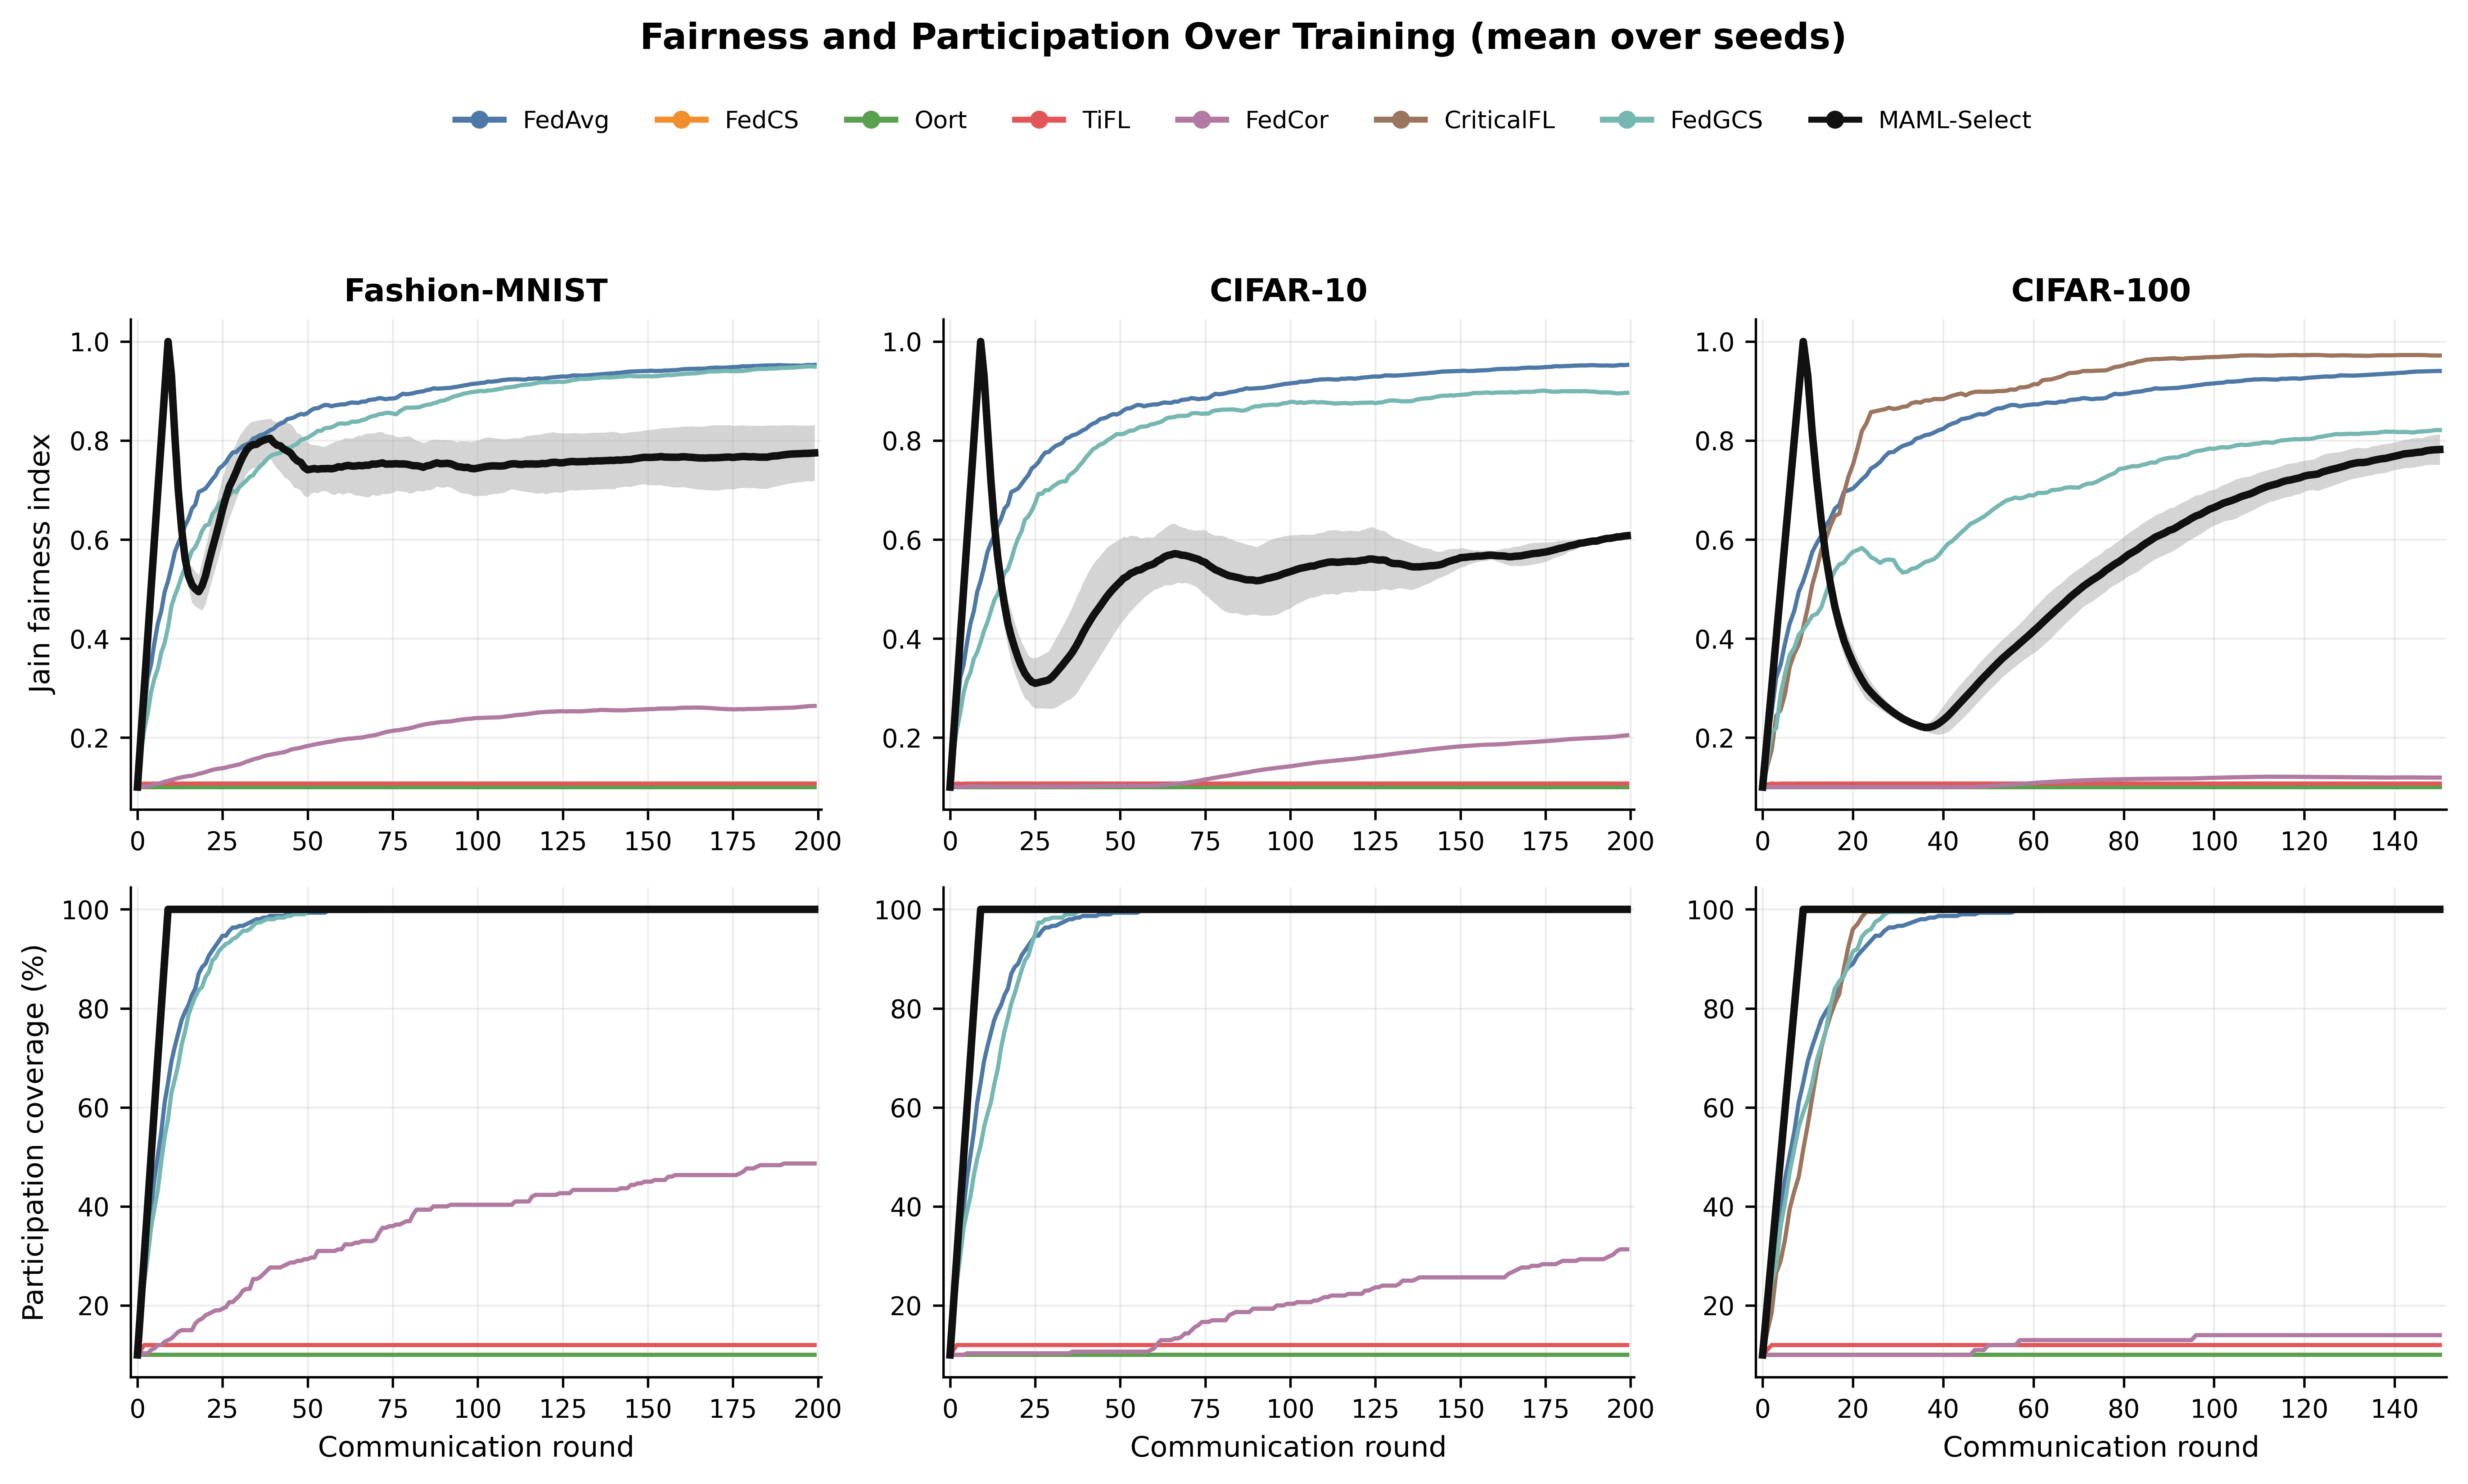
\includegraphics[width=0.98\textwidth]{supp_fairness_trajectories.png}
\caption{Jain fairness index (top) and participation-coverage ratio (bottom) versus round. MAML-Select reaches full ($100\%$) client coverage like FedAvg and FedGCS, but its Jain index settles below them; the system-aware baselines that always pick the fastest tier (FedCS, Oort, TiFL) stay near $10$--$12\%$ coverage. This is the transparent basis for not claiming fairness superiority.}
\label{fig:supp_fairness_traj}
\end{figure}

\begin{figure}[!ht]
\centering
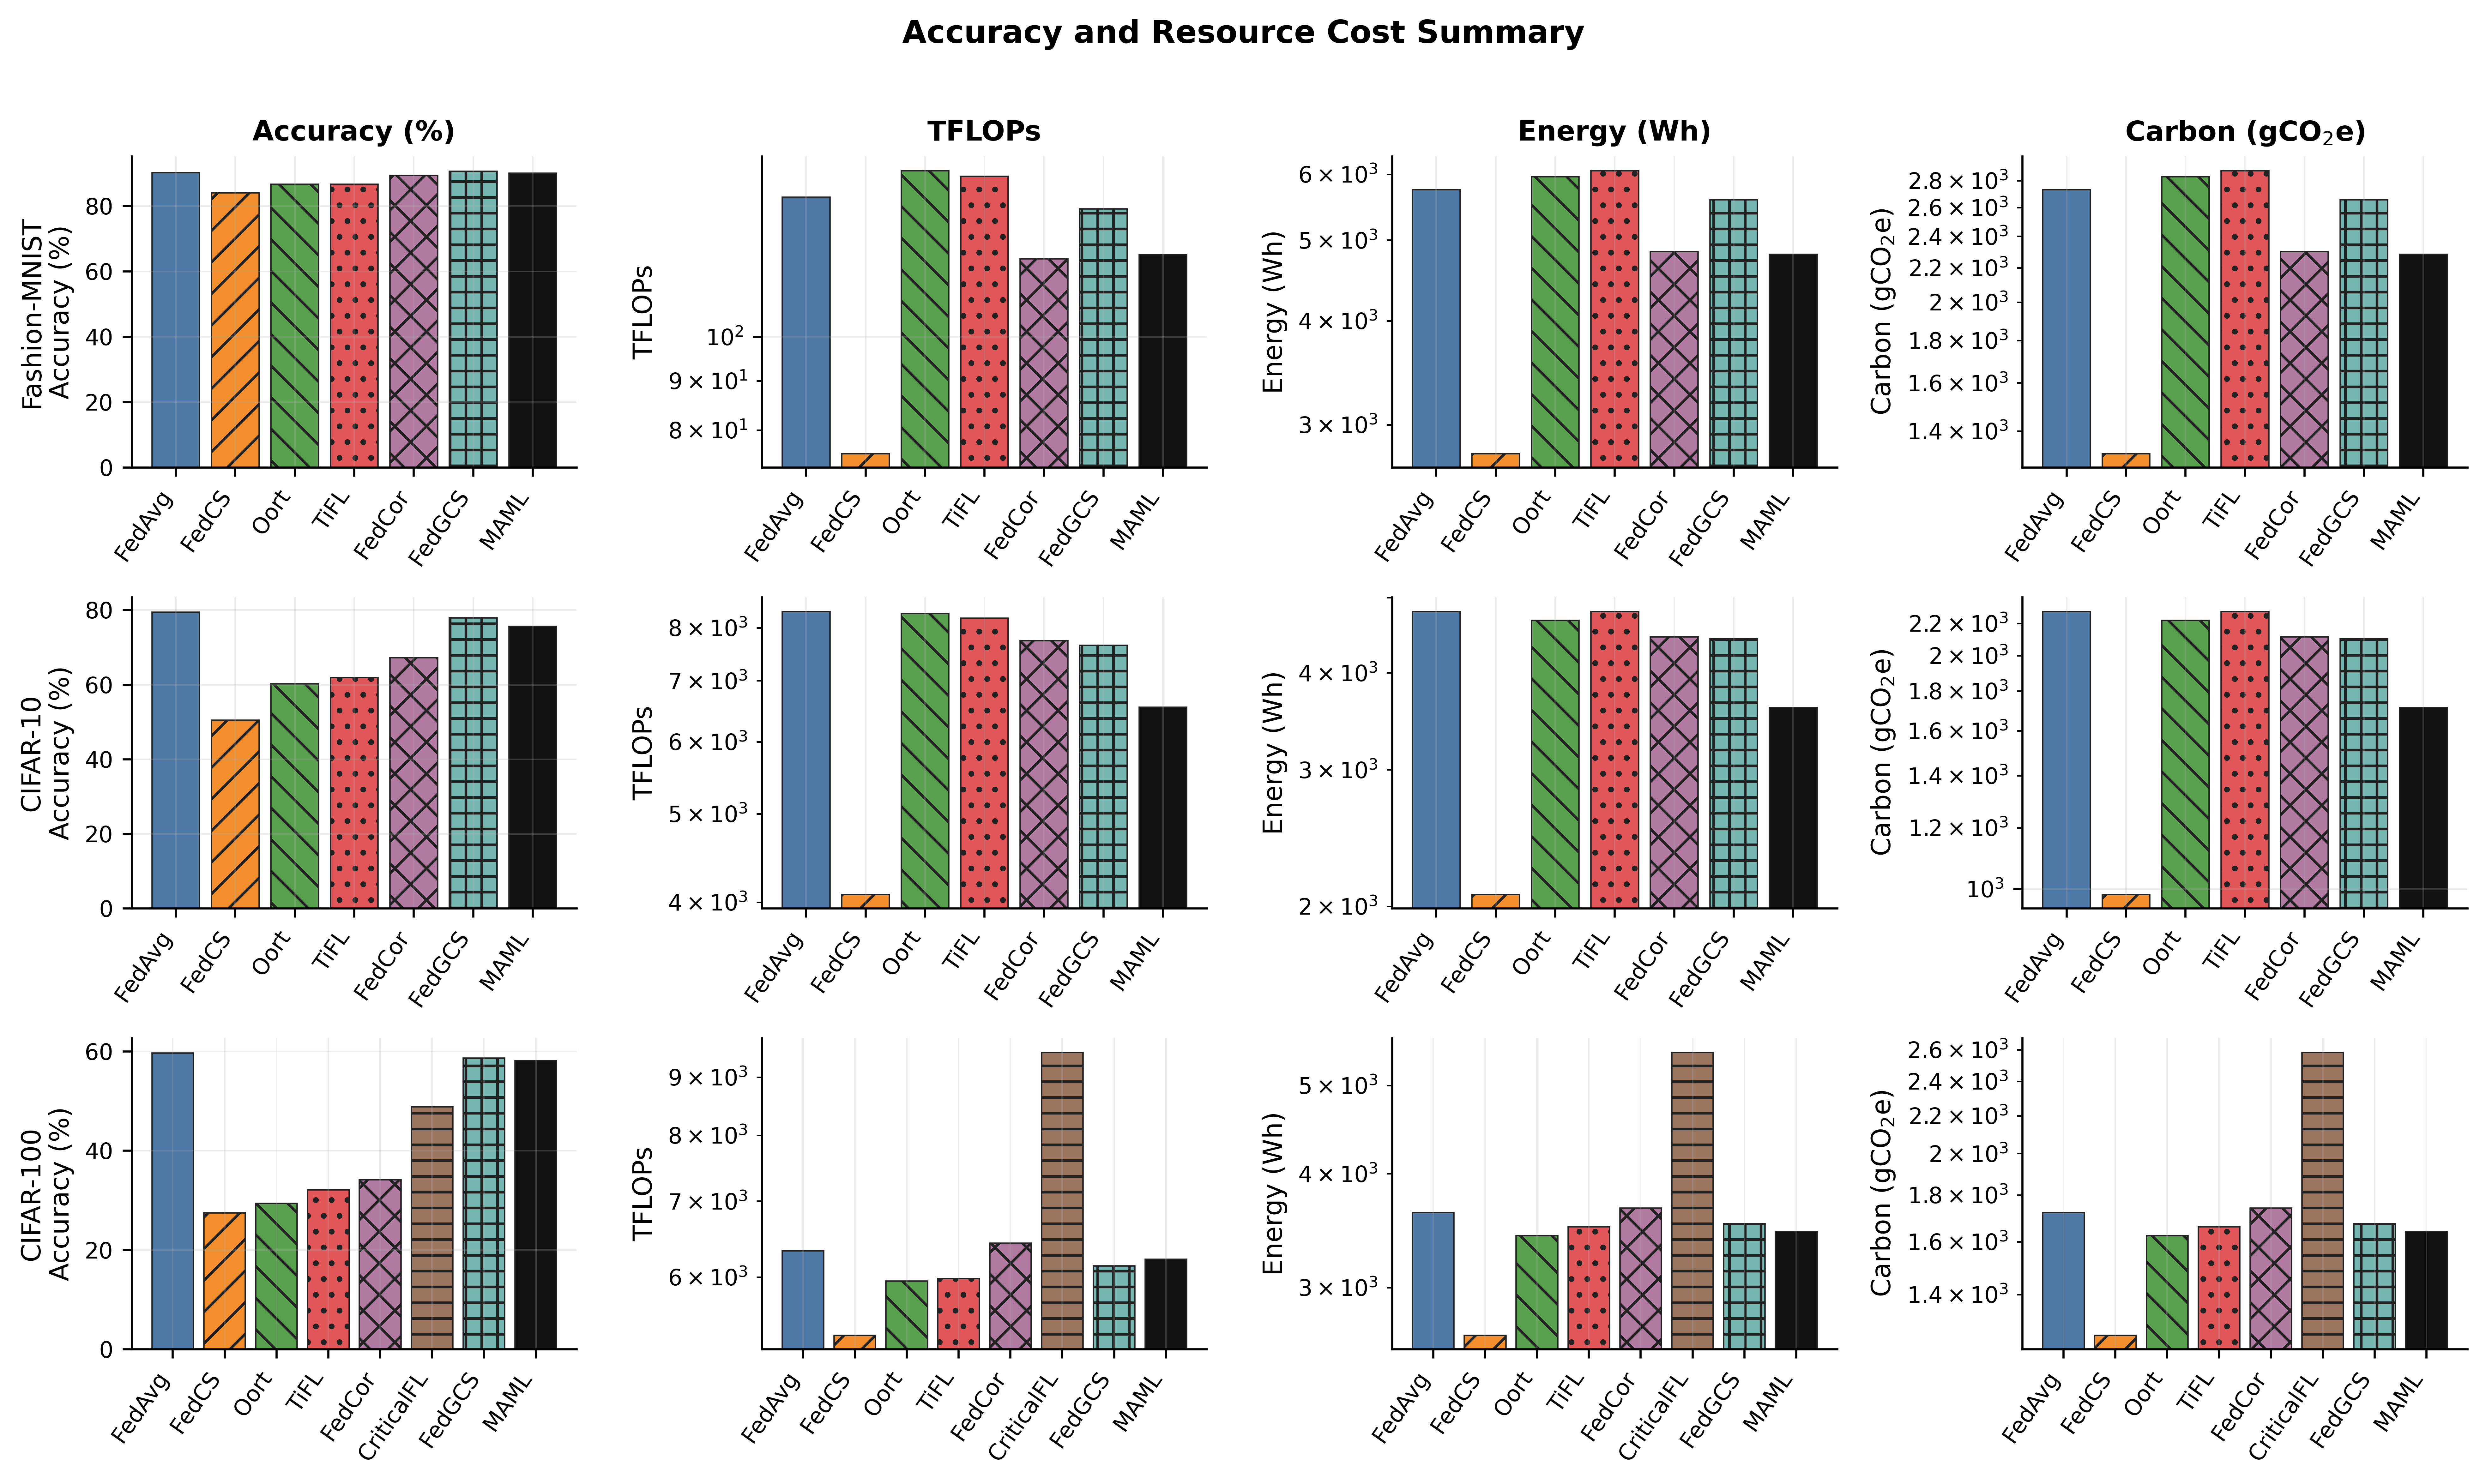
\includegraphics[width=0.96\textwidth]{review_fig_efficiency_resource_grid.png}
\caption{Expanded accuracy/resource grid across datasets and methods, retained as supplementary evidence. The main letter reports the same information more compactly through the benchmark table and the trade-off figure.}
\label{fig:supp_resource_grid}
\end{figure}

\begin{figure}[!ht]
\centering
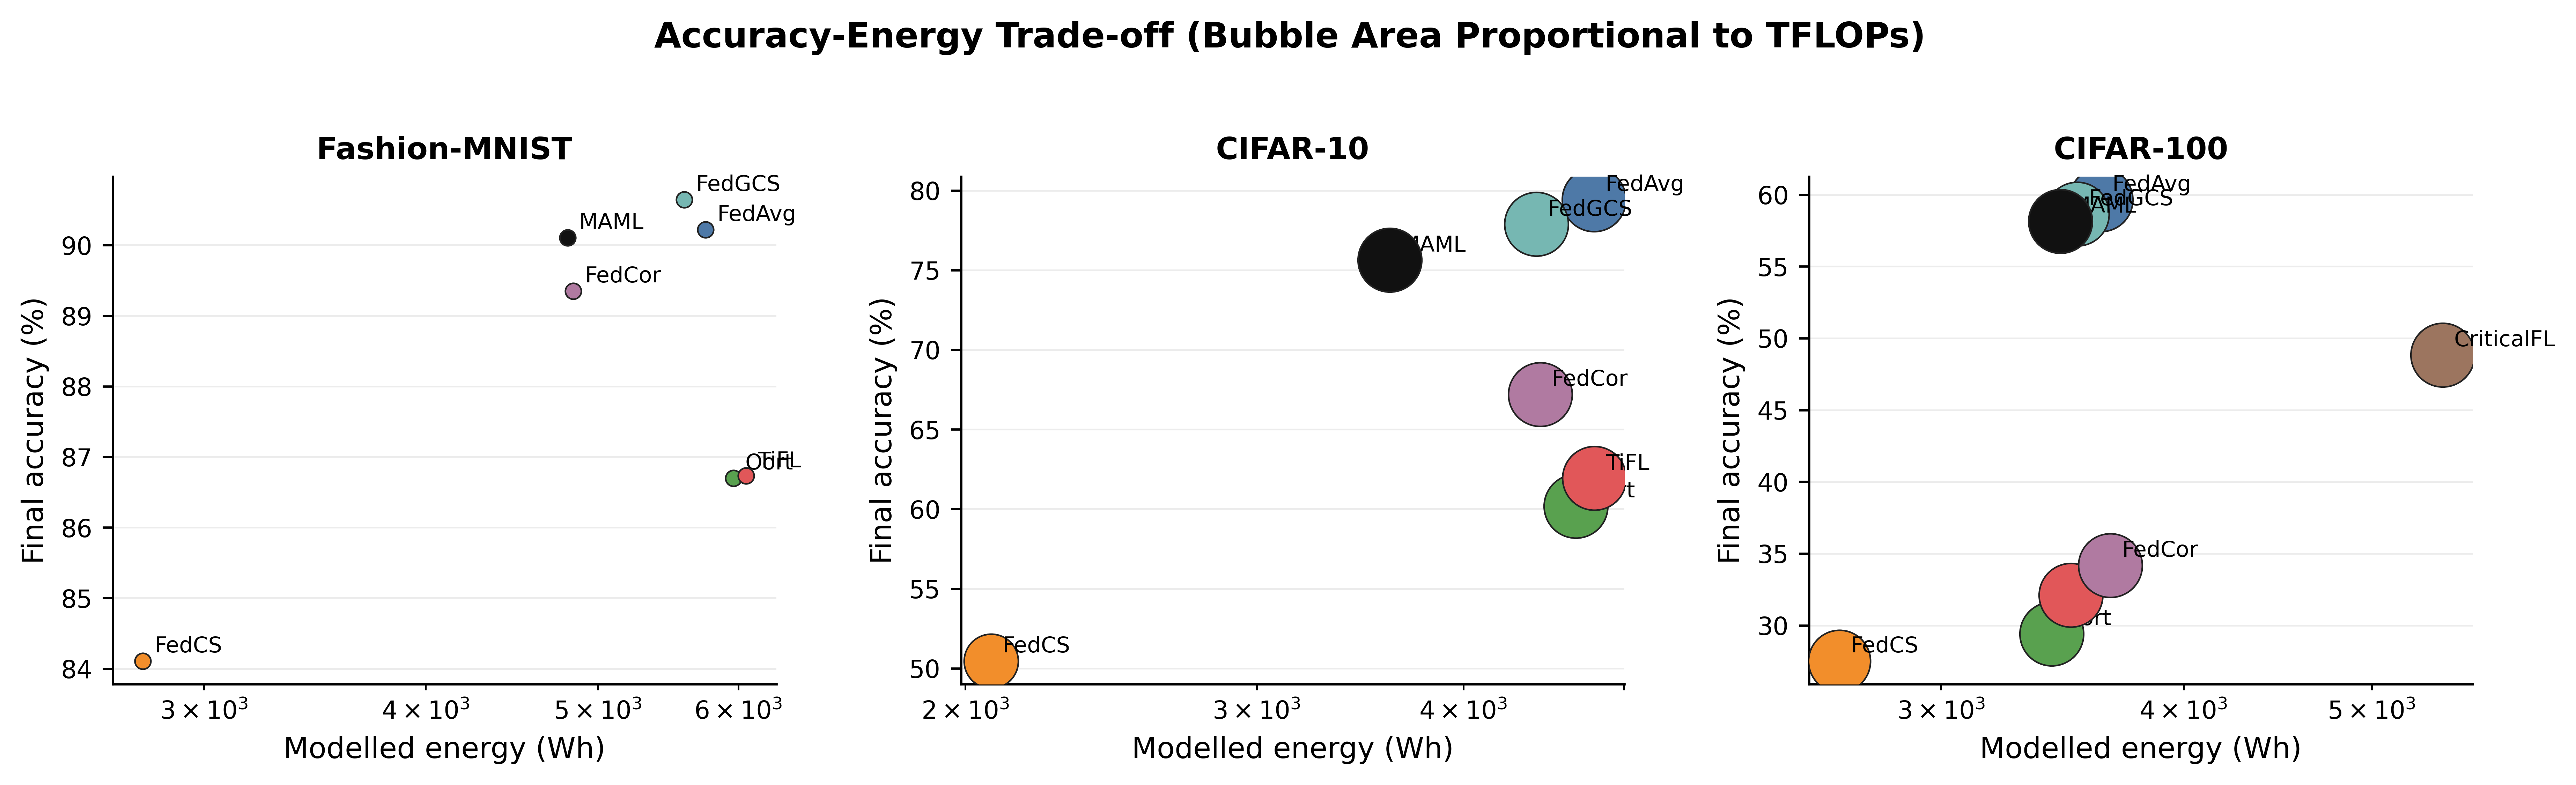
\includegraphics[width=0.74\textwidth]{review_fig_accuracy_energy_tradeoff.png}
\caption{Accuracy--energy trade-off view used as a cross-check for the final normalized trade-off plot. The main paper uses the normalized compute view because communication is identical across selectors and the TFLOP axis is easier to compare across datasets.}
\label{fig:supp_accuracy_energy}
\end{figure}

\section*{S6. Efficiency Frontier and Reproducibility}

Figure~\ref{fig:supp_pareto} places every method on the accuracy-versus-cost plane; MAML-Select (star) sits toward the favorable upper-left region---competitive accuracy at lower modeled energy and compute---on Fashion-MNIST and CIFAR-100, and trades accuracy for cost on CIFAR-10. Figure~\ref{fig:supp_repro} shows the underlying per-seed accuracies, evidencing tight run-to-run dispersion for MAML-Select.

\begin{figure}[!ht]
\centering
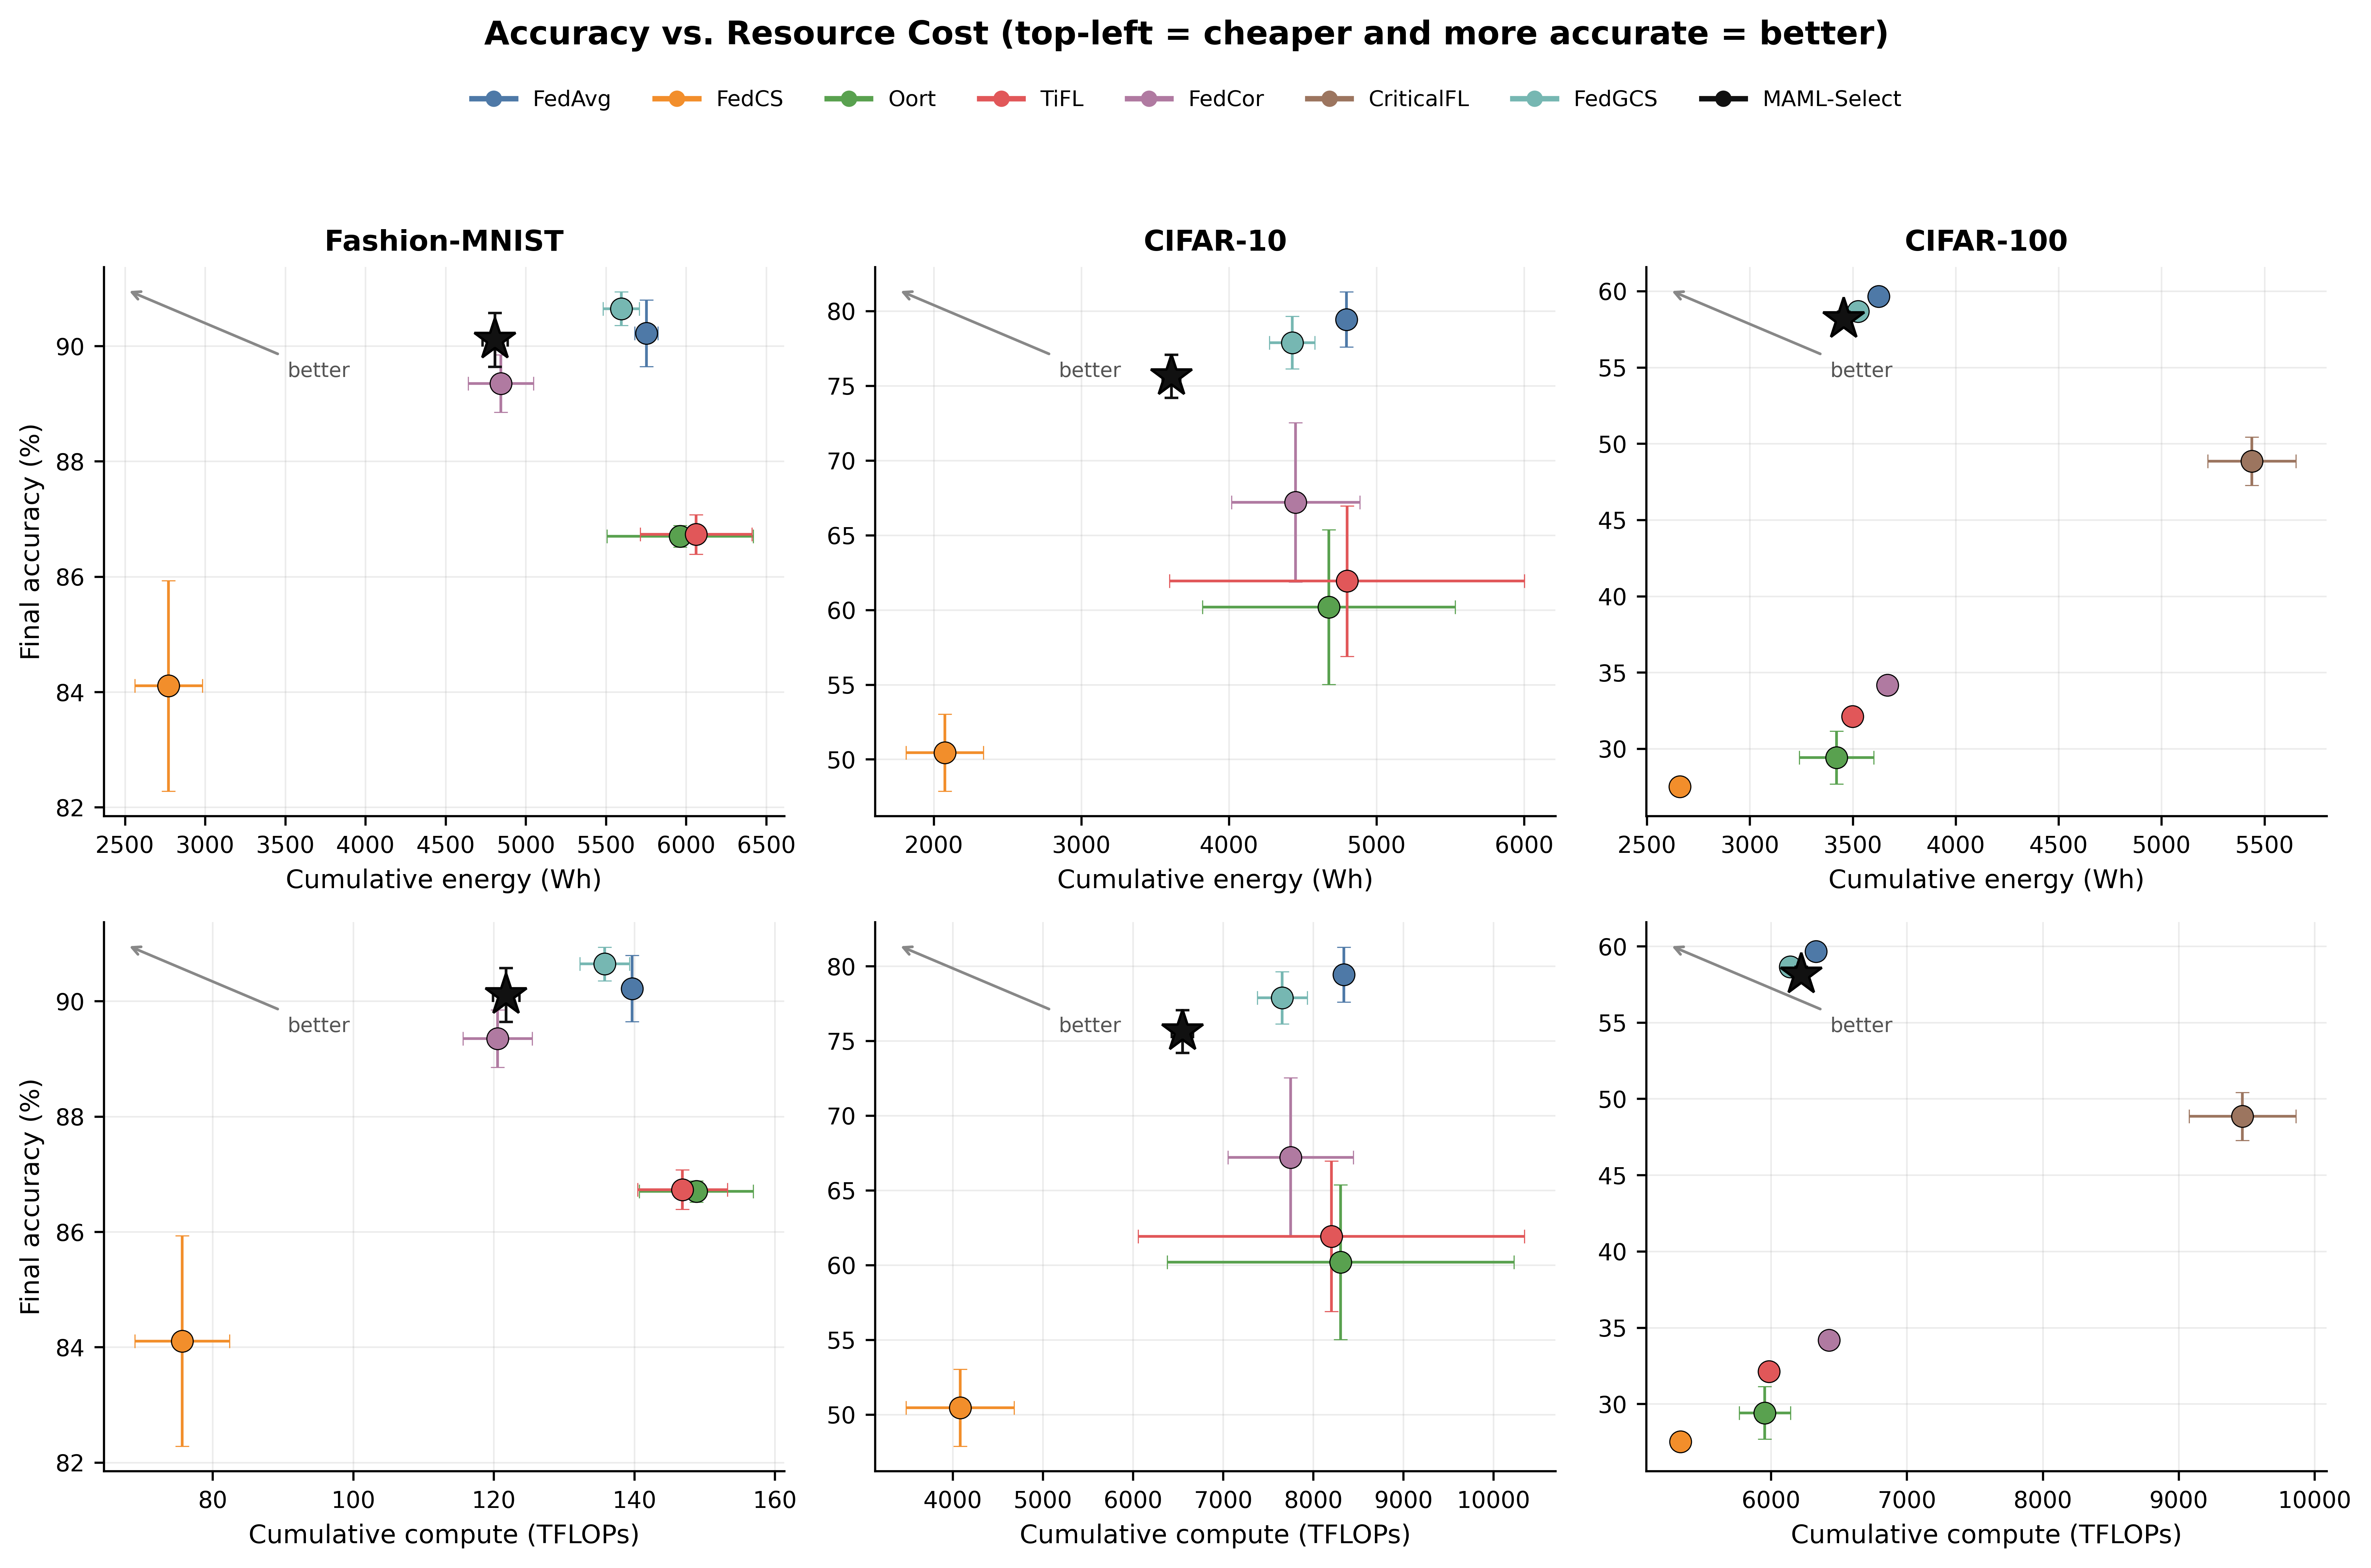
\includegraphics[width=0.98\textwidth]{supp_pareto_fronts.png}
\caption{Accuracy versus cumulative energy (top) and cumulative compute (bottom). Markers are seed means with $\pm1$~s.d.\ error bars; the upper-left direction (cheaper and more accurate) is better. MAML-Select (star) lies on or near the efficient frontier on Fashion-MNIST and CIFAR-100 and reflects the explicit accuracy trade-off on CIFAR-10.}
\label{fig:supp_pareto}
\end{figure}

\begin{figure}[!ht]
\centering
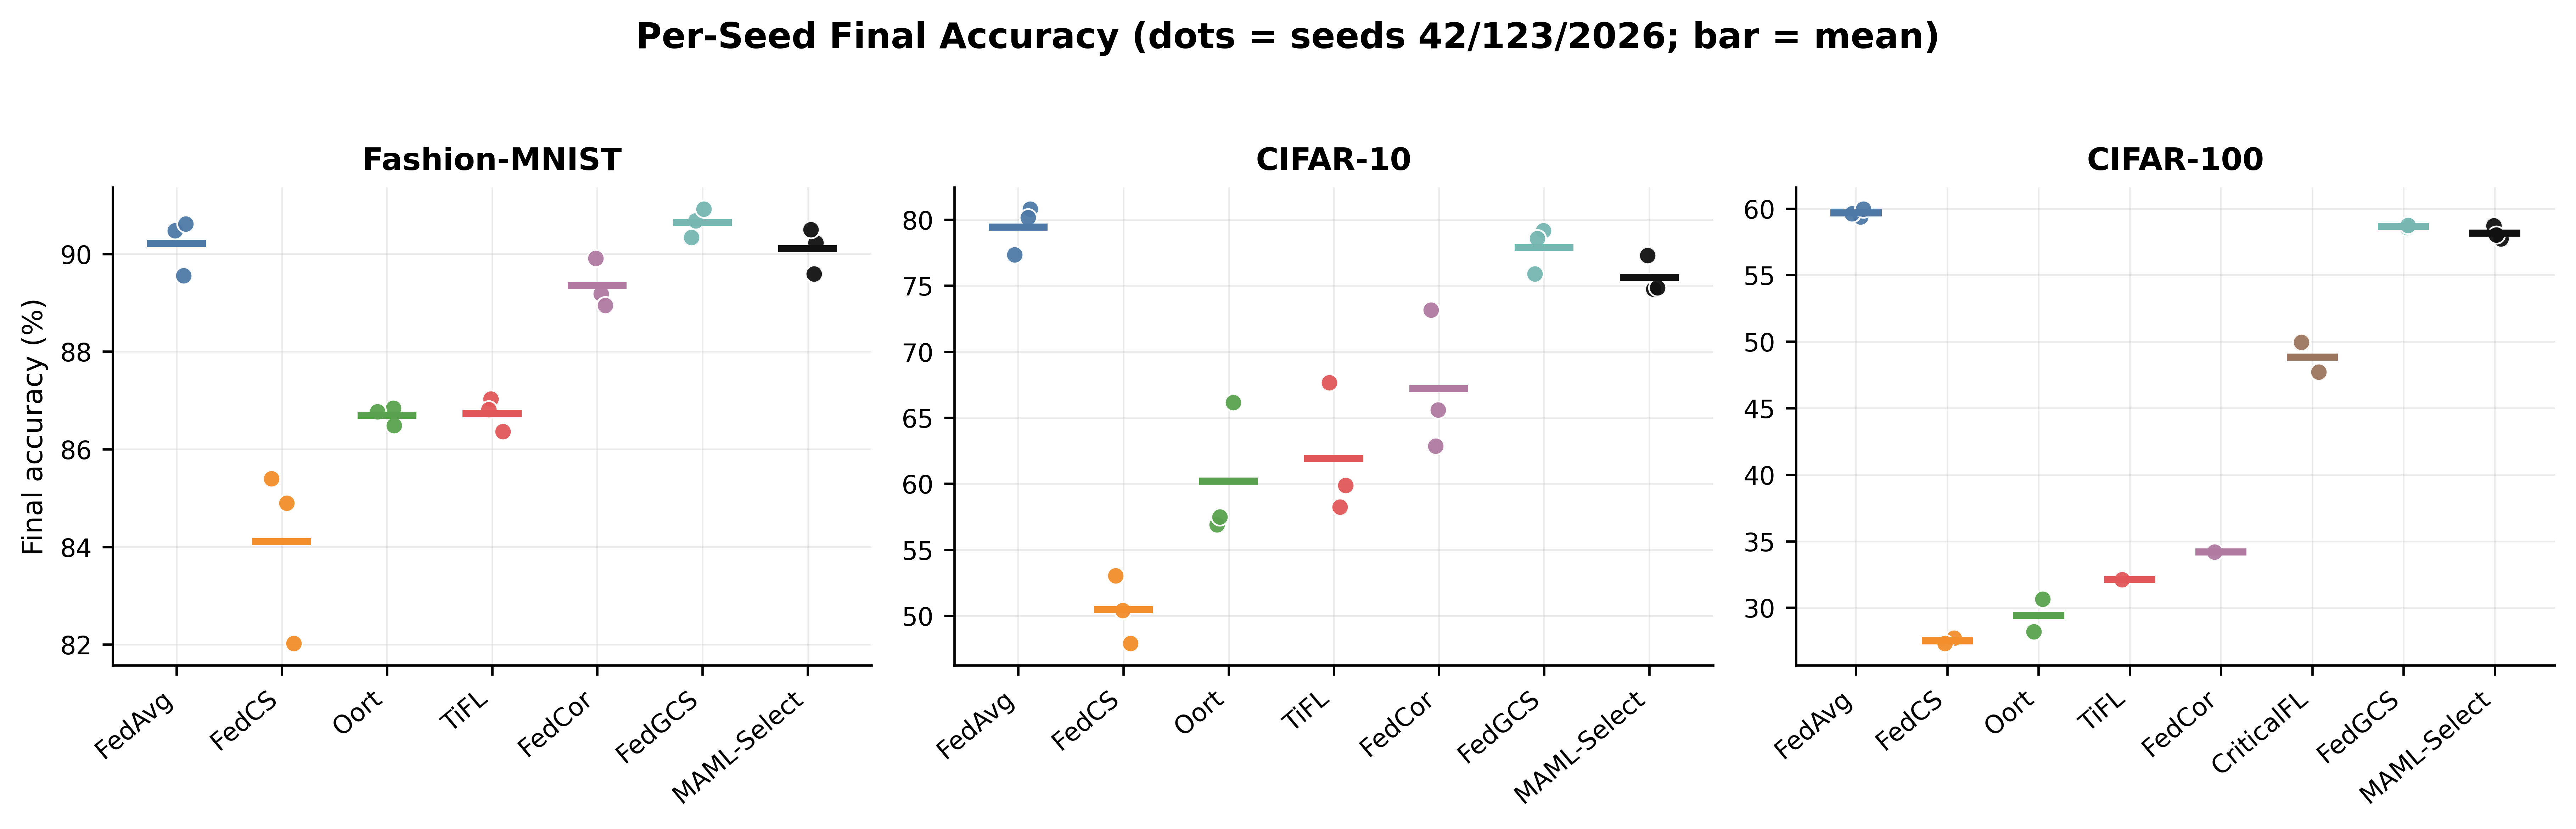
\includegraphics[width=0.98\textwidth]{supp_reproducibility_seeds.png}
\caption{Per-seed final accuracy (dots: seeds $42$, $123$, $2026$; bar: mean). MAML-Select's spread is small on Fashion-MNIST and CIFAR-100 and moderate on CIFAR-10; CriticalFL appears only for CIFAR-100, consistent with its incomplete Fashion-MNIST and CIFAR-10 runs.}
\label{fig:supp_repro}
\end{figure}

\section*{S7. Sensitivity, Ablation, and Overhead}

\begin{figure}[!ht]
\centering
\begin{minipage}{0.49\textwidth}
\centering

\includegraphics[width=\linewidth]{review_fig_lambda_sensitivity.png}
\caption*{(a) $\lambda$ sensitivity.}
\end{minipage}
\hfill
\begin{minipage}{0.49\textwidth}
\centering

\includegraphics[width=\linewidth]{review_fig_feature_ablation.png}
\caption*{(b) State-feature ablation.}
\end{minipage}
\caption{Design-analysis plots on Fashion-MNIST. The selected operating point is $\lambda=0.5$. Accuracy remains stable over the sweep, while larger $\lambda$ reduces compute, energy, and carbon at the cost of participation fairness.}
\label{fig:supp_lambda_ablation_side}
\end{figure}

\begin{table}[!ht]
\centering
\caption{$\lambda$ sensitivity on Fashion-MNIST ($n=3$). Accuracy is reported as mean $\pm$ s.d.; remaining columns are means.}
\label{tab:supp_lambda}
\small
\begin{tabular}{@{}lrrrrr@{}}
\toprule
$\lambda$ & Acc. (\%) & TFLOPs & Energy (Wh) & Carbon (g) & Jain \\
\midrule
0.1 & $90.40 \pm 0.22$ & 128.3 & 5176 & 2459 & 0.91 \\
0.5 & $90.23 \pm 0.55$ & 121.6 & 4799 & 2280 & 0.78 \\
1.0 & $89.74 \pm 0.79$ & 118.6 & 4639 & 2204 & 0.71 \\
5.0 & $89.37 \pm 1.02$ & 107.8 & 4140 & 1966 & 0.50 \\
\bottomrule
\end{tabular}
\end{table}

\begin{table}[!ht]
\centering
\caption{State-feature ablation on Fashion-MNIST ($n=3$). Each row removes one feature from the six-dimensional MAML-Select state vector.}
\label{tab:supp_ablation}
\small
\begin{tabular}{@{}lrrrr@{}}
\toprule
Variant & Acc. (\%) & TFLOPs & Energy (Wh) & Jain \\
\midrule
Full state vector & $90.23 \pm 0.55$ & 121.6 & 4799 & 0.78 \\
w/o loss & $90.16 \pm 0.66$ & 122.8 & 4851 & 0.79 \\
w/o gradient norm & $90.30 \pm 0.24$ & 122.4 & 4831 & 0.78 \\
w/o latency & $90.14 \pm 0.14$ & 118.9 & 4688 & 0.70 \\
w/o battery & $89.90 \pm 0.44$ & 122.2 & 4830 & 0.79 \\
w/o frequency & $90.47 \pm 0.13$ & 115.0 & 4533 & 0.65 \\
w/o staleness & $90.37 \pm 0.19$ & 122.7 & 4838 & 0.78 \\
\bottomrule
\end{tabular}
\end{table}

\begin{figure}[!ht]
\centering
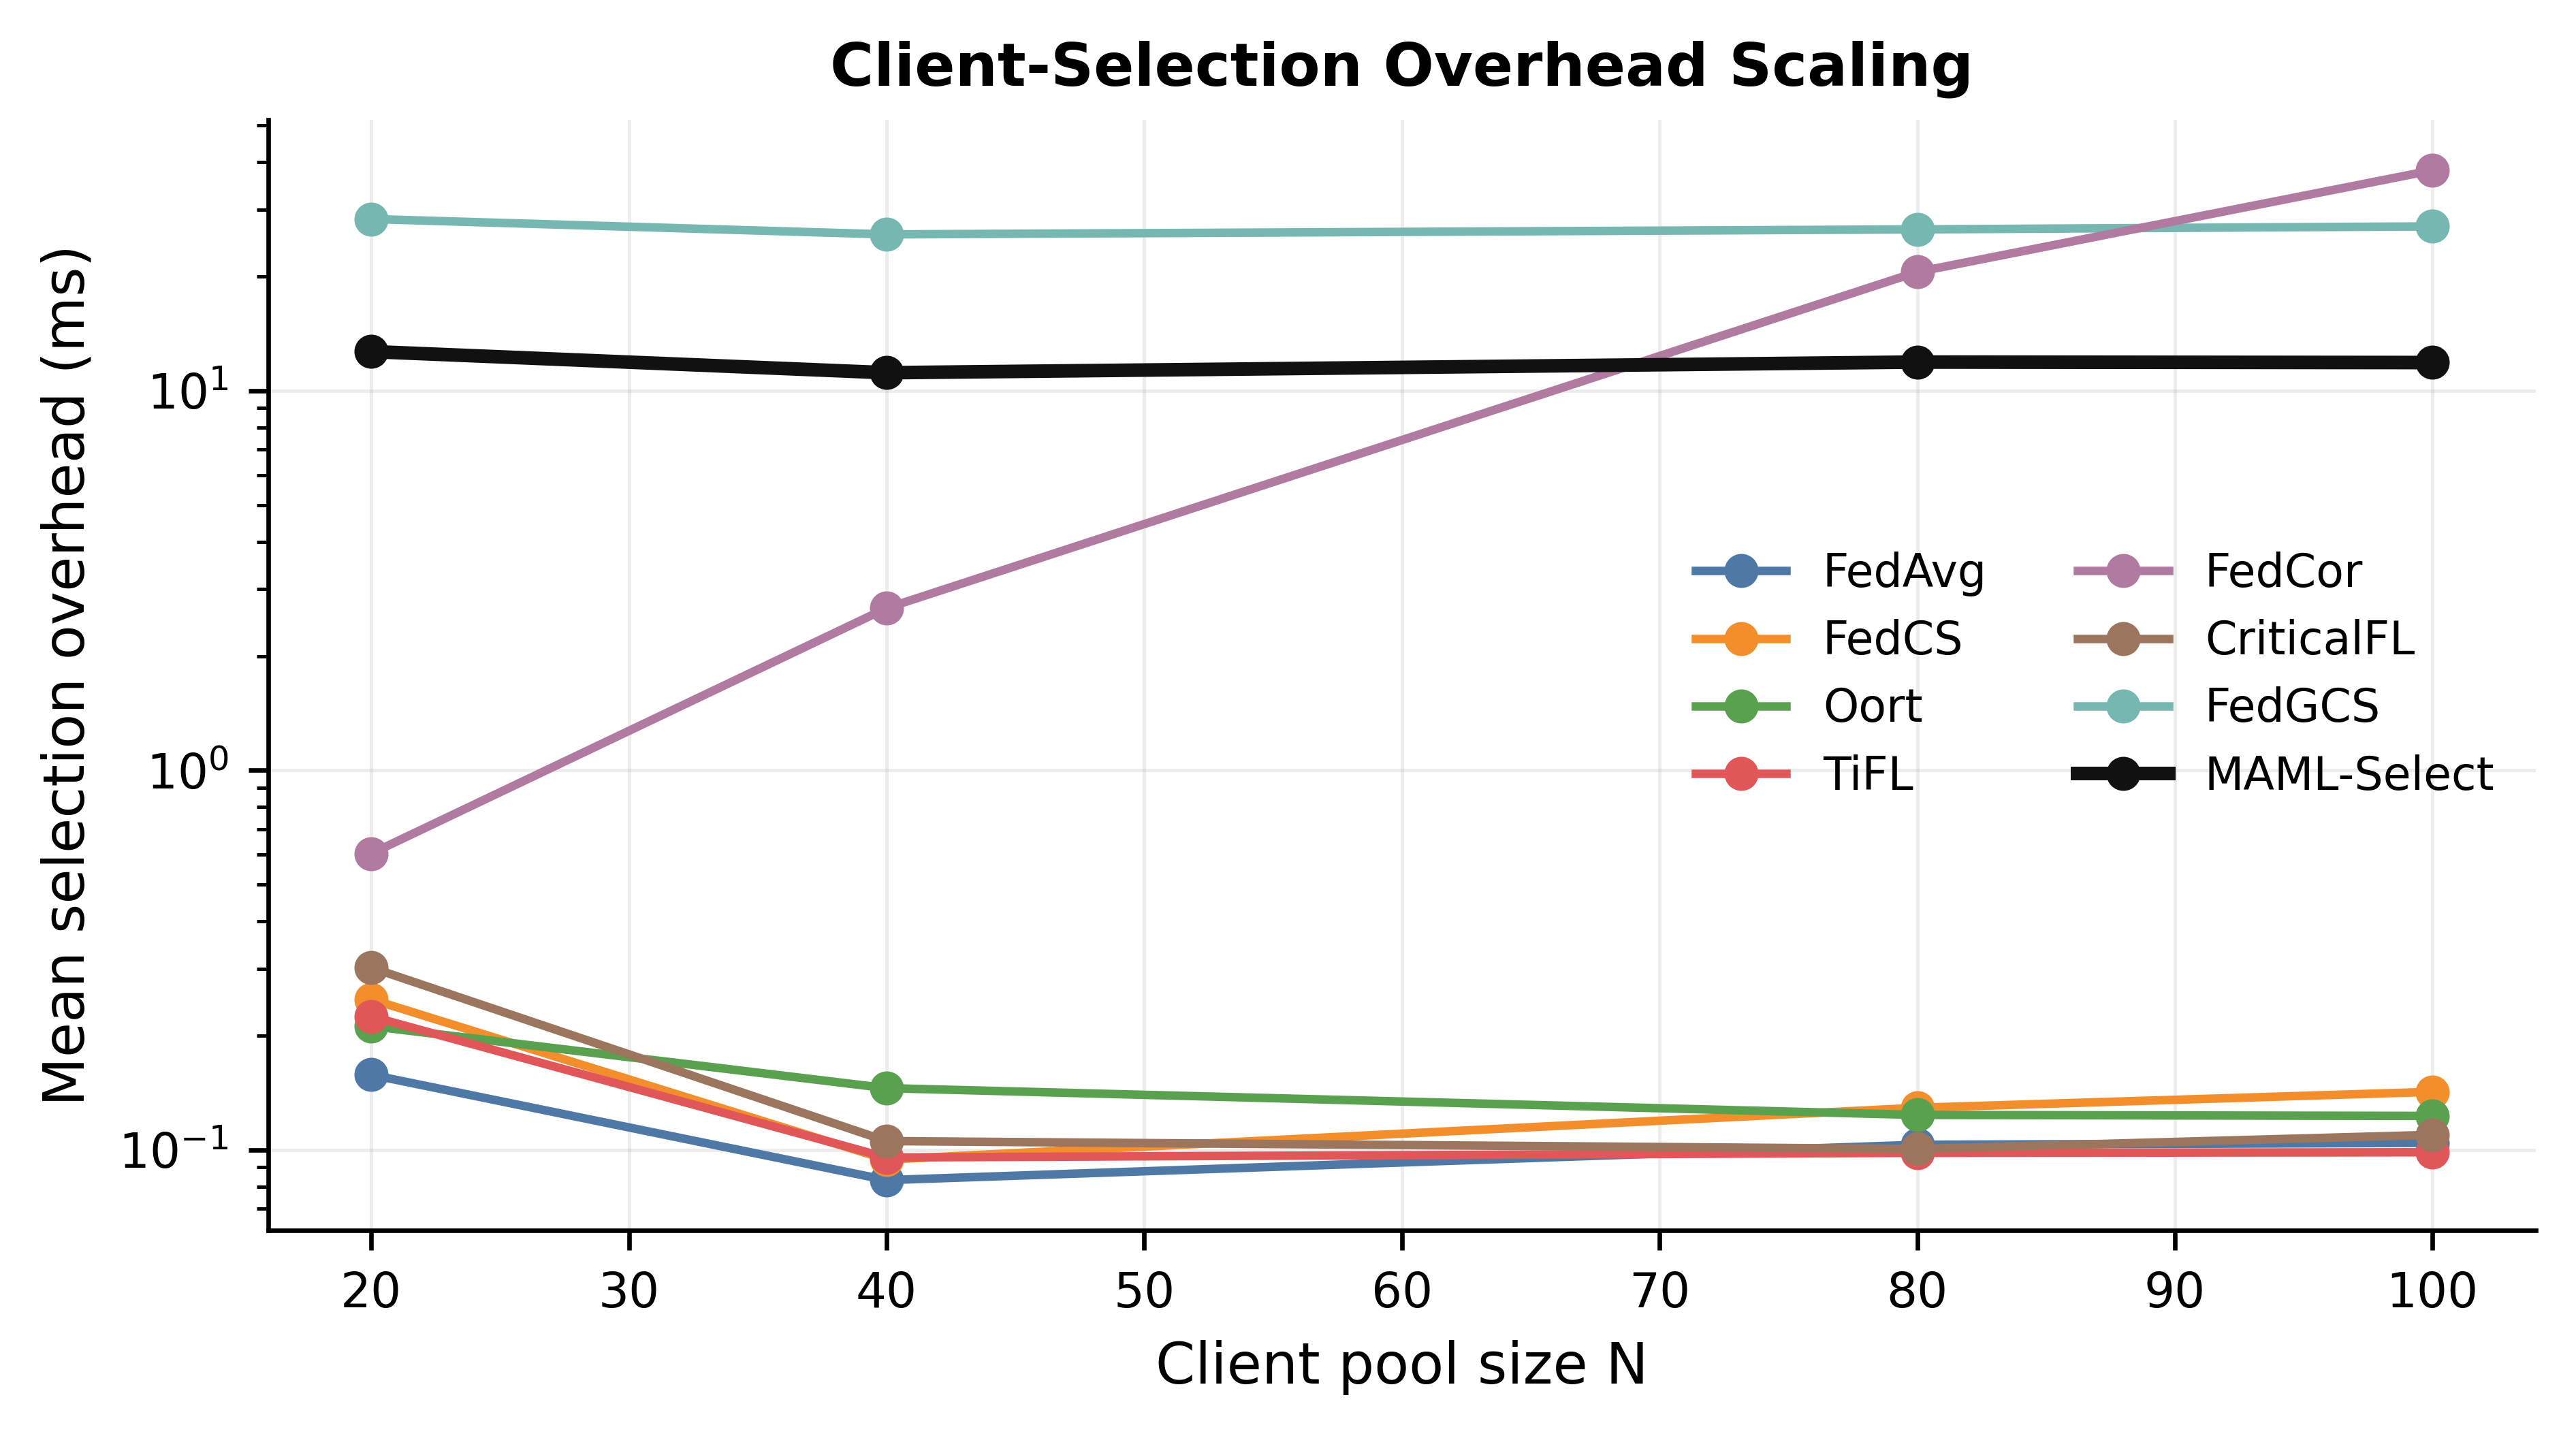
\includegraphics[width=0.74\textwidth]{review_fig_scaling_overhead.png}
\caption{Selector overhead scaling with the client-pool size $N$. MAML-Select's per-round selection time stays in the $11$--$13$~ms range and is dominated by local training; only FedCor grows steeply with $N$.}
\label{fig:supp_scaling}
\end{figure}

\begin{table}[!ht]
\centering
\caption{Mean client-selection overhead in seconds for the scaling probe (10 rounds per setting).}
\label{tab:supp_scaling}
\small
\begin{tabular}{@{}lrrrr@{}}
\toprule
Method & $N=20$ & $N=40$ & $N=80$ & $N=100$ \\
\midrule
FedAvg & 0.000158 & 0.000083 & 0.000103 & 0.000104 \\
FedCor & 0.000604 & 0.002676 & 0.020562 & 0.038099 \\
FedGCS & 0.028355 & 0.025831 & 0.026627 & 0.027116 \\
MAML-Select & 0.012689 & 0.011160 & 0.011907 & 0.011871 \\
\bottomrule
\end{tabular}
\end{table}

\section*{S8. Limitations and Threats to Validity}

We state the boundaries of the evidence plainly. (i) \textbf{Modeled, not metered, energy.} Energy and carbon are derived from the device-tier power model and a single declared grid intensity ($475$~g\,CO$_2$/kWh); they are consistent, reproducible estimates rather than hardware-meter readings, and absolute Wh/g values would shift under a different tier model or grid. (ii) \textbf{Three seeds.} All confidence intervals and effect sizes are computed at $n=3$ (fewer where runs are incomplete), so the intervals are wide; we therefore lead with effect sizes and report $n$ in every table. (iii) \textbf{Fairness.} MAML-Select reaches full client coverage but its Jain index is below FedAvg and FedGCS on all datasets; we report this rather than claim a fairness benefit. (iv) \textbf{Single non-IID regime.} Experiments use one Dirichlet setting ($\alpha=0.5$) and one $100$-client, three-tier topology; broader heterogeneity and scale are left to future work. (v) \textbf{Incomplete baseline coverage.} CriticalFL completed only on CIFAR-100; its missing Fashion-MNIST and CIFAR-10 entries are left blank rather than estimated.

\section*{S9. Interpretation for the Revised Claims}

The supplementary results support three cautious claims. First, MAML-Select is not presented as a universal accuracy winner; it is competitive with FedAvg and FedGCS on Fashion-MNIST and CIFAR-100 while reducing modeled resource use, and it makes an explicit, quantified accuracy concession on CIFAR-10. Second, the resource estimates follow the stated simulator assumptions for device tiers and grid intensity (S2), and the savings accumulate consistently across training (S5) with large paired effect sizes (S4). Third, fairness is reported explicitly: MAML-Select reaches full client coverage but its Jain index is lower than FedAvg and FedGCS, so the manuscript avoids claiming fairness superiority. Taken together, the enhanced supplement substantiates the efficiency-and-adaptivity contribution of the method while being transparent about its costs.

\end{document}
